\documentclass[border=10pt]{standalone}

\usepackage{tikz}
\usepackage{tikzsymbols}
\usetikzlibrary{calc,patterns,shapes.geometric}

\def\centerarc[#1](#2)(#3:#4:#5){\draw[#1] ($(#2)+({#5*cos(#3)},{#5*sin(#3)})$) arc (#3:#4:#5);}

\begin{document}
	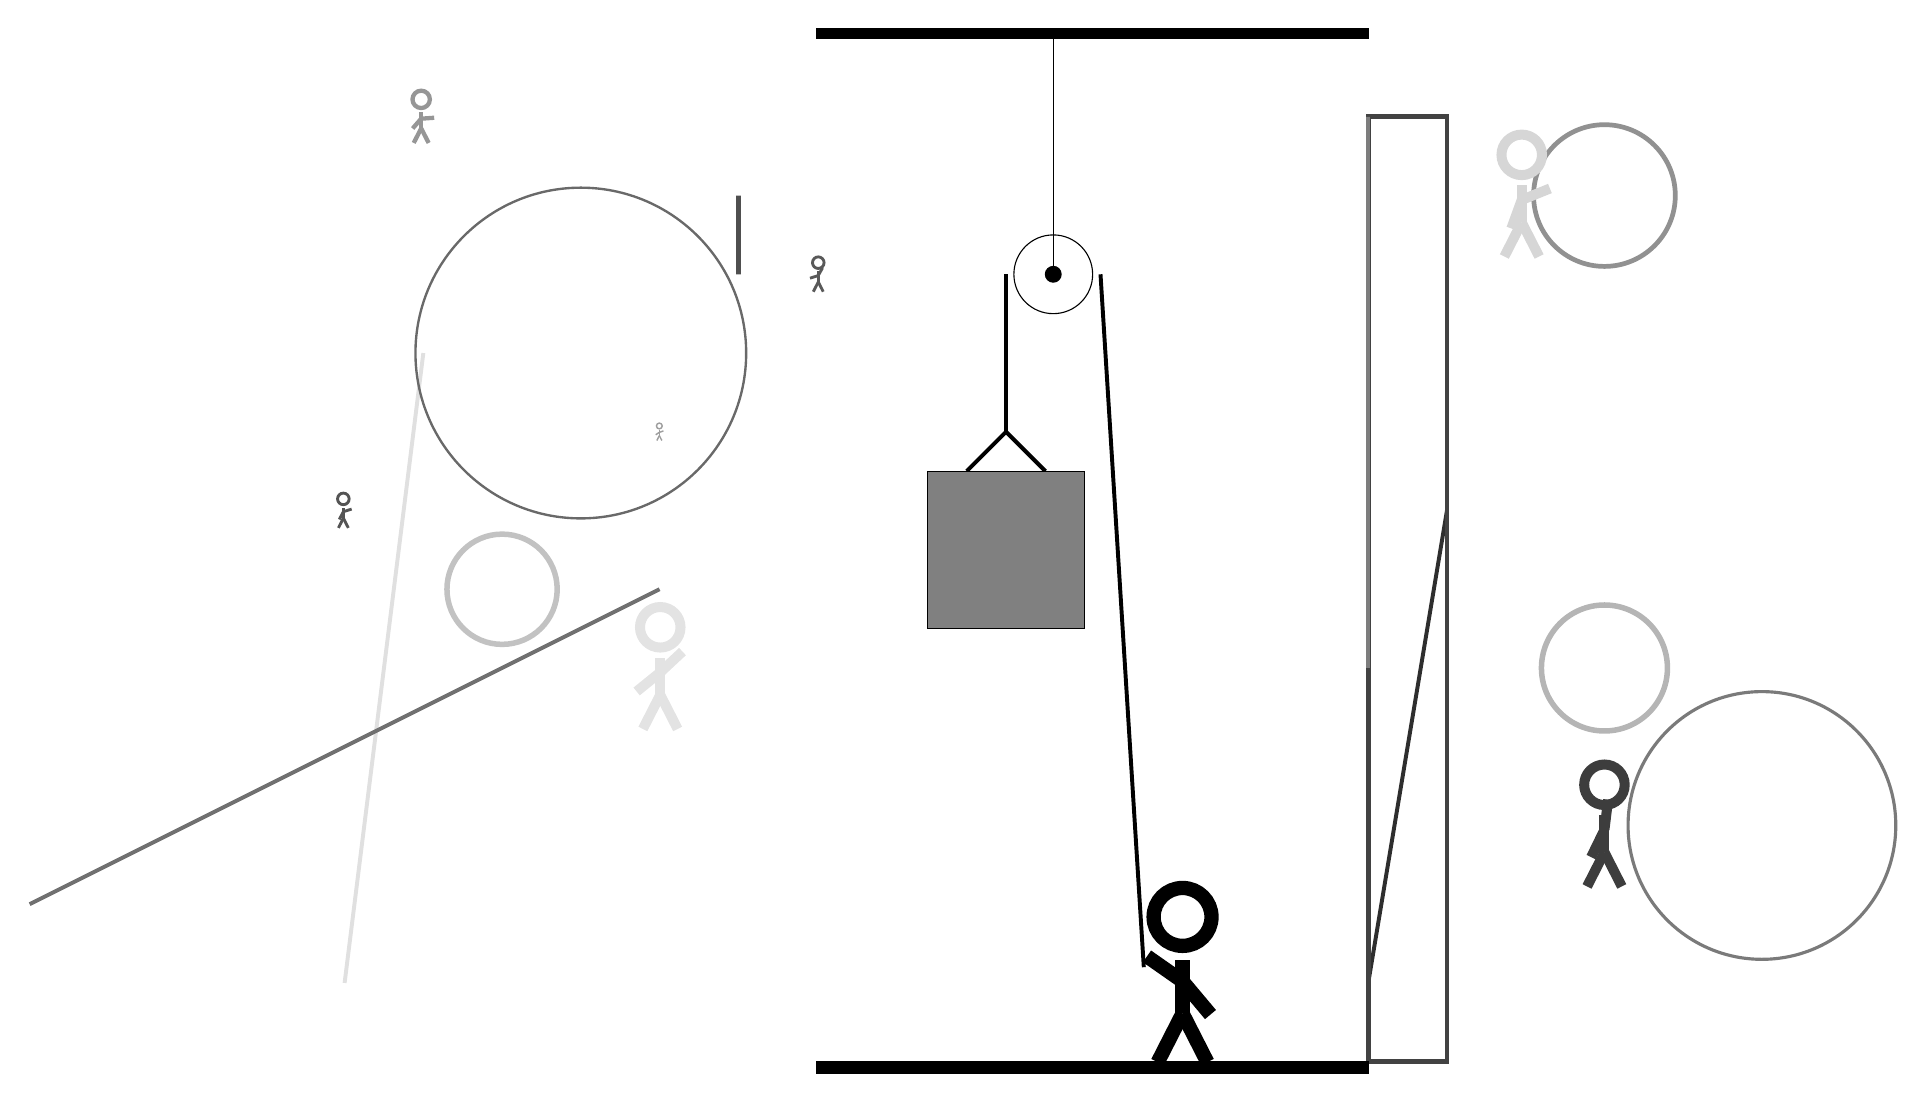
\begin{tikzpicture}
		%%%%% START %%%%%
		
		\draw[fill=black] (-2, 10) rectangle (5, 10.125);
		
		\draw (1, 7) circle (0.5);
		\draw[fill=black] (1, 7) circle (0.1);
		\draw (1, 10) -- (1, 7);
		
		\draw [line width=0.6mm, color=black!43](8, 8) circle (0.9);
		
		\draw[line width=0.5mm, color=black!82](6, 4) -- (5, -2);
		\draw [line width=0.4mm, color=black!52](10, 0) circle (1.7);
		\node[line width=0.7mm, color=black!65] at (-2, 7) {\Strichmaxerl[2][18][61]};
		\draw[line width=0.5mm, color=black!12](-7, 6) -- (-8, -2);
		
		\node[line width=0.3mm, color=black!16] at (7, 8) {\Strichmaxerl[7][70][22]};
		
		\node[line width=0.5mm, color=black!11] at (-4, 2) {\Strichmaxerl[7][39][43]};
		\draw[line width=0.5mm, color=black!56](-4, 3) -- (-12, -1);
		\draw [line width=0.7mm, color=black!24](-6, 3) circle (0.7);
		
		\draw[line width=0.6mm, color=black!74] (5, -3) rectangle (6, 9);
		\draw [line width=0.3mm, color=black!59](-5, 6) circle (2.1);
		
		\node[line width=0.6mm, color=black!41] at (-7, 9) {\Strichmaxerl[3][49][4]};
		\draw[line width=0.7mm, color=black!69] (-3, 7) rectangle (-3, 8);
		\node[line width=0.5mm, color=black!76] at (8, 0) {\Strichmaxerl[7][64][83]};
		\draw [line width=0.7mm, color=black!29](8, 2) circle (0.8);
		\draw[line width=0.5mm, color=black!51] (5, 9) rectangle (5, 2);
		
		\node[line width=0.3mm, color=black!38] at (-4, 5) {\Strichmaxerl[1][33][20]};
		\node[line width=0.2mm, color=black!67] at (-8, 4) {\Strichmaxerl[2][62][18]};
		
		\draw[line width=0.5mm] (-0.1, 4.5) -- (0.4, 5.0) -- (0.9, 4.5);
		\draw[fill=black!50] (-0.6, 4.5) rectangle (1.4, 2.5);
		
		\draw[line width=0.5mm] (0.4, 7) -- (0.4, 5.0);
		\centerarc[line width=0.5mm](1, 7)(0:180:0.6);
		\draw[line width=0.5mm](1.6, 7) -- (2.15, -1.8);
		
		\node at (2.6, -1.9) {\Strichmaxerl[10][-35][-50]};
		
		\draw[fill=black] (-2, -3) rectangle (5, -3.15);
		
		%%%%% END %%%%%
	\end{tikzpicture}
\end{document}